\documentclass[11pt]{article}
\usepackage[T1]{fontenc}
\usepackage[margin=1in]{geometry}
\usepackage{amsmath,amssymb,amsthm,mathtools}
\usepackage{booktabs}
\usepackage{graphicx}
\usepackage{microtype}
\usepackage{xcolor}
\usepackage[colorlinks=true,linkcolor=blue!55!black,urlcolor=blue!65!black]{hyperref}

\newtheorem{theorem}{Theorem}
\newtheorem{corollary}[theorem]{Corollary}
\newtheorem{proposition}[theorem]{Proposition}
\newcommand{\E}{\mathcal E}
\newcommand{\R}{\mathbb R}

\title{Equal spherical droplets are exactly optimal\
within the spherical-fragmentation class}
\author{Candidate substantial partial answer to Conjecture 6.1\
in arXiv:1004.4271}
\date{11 August 2026}

\begin{document}
\maketitle

\begin{center}
\fbox{\begin{minipage}{0.91\textwidth}
\textbf{Status: candidate substantial partial result, likely valid.}
For the three-dimensional liquid-drop ball energy, the minimum over every
finite or countable mass fragmentation is always an equal fragmentation.
The optimal number of droplets and every transition mass are explicit, and
the equal state is strictly stable under mass-preserving perturbations away
from transitions. Consequently the conjectured formula is exact over finite
unions of spherical components. The unrestricted arbitrary-shape conjecture
remains open.
\end{minipage}}
\end{center}

\section{Source question and the restricted result}

Choksi and Peletier study the three-dimensional liquid-drop energy
\[
 e_0(m)=\inf_{|\Omega|=m}\left\{
 P(\Omega)+\iint_{\Omega\times\Omega}
 \frac{dx\,dy}{4\pi|x-y|}\right\}.
\]
For a ball of volume $s$, its value is
\begin{equation}\label{eq:f}
 f(s)=a s^{2/3}+b s^{5/3},\qquad
 a=(36\pi)^{1/3},\quad
 b=\frac25\left(\frac3{4\pi}\right)^{2/3},
 \quad \frac ab=10\pi.
\end{equation}
Conjecture 6.1 of arXiv:1004.4271 proposes, among other assertions,
\begin{equation}\label{eq:source-envelope}
 e_0(m)=\inf_{n\in\mathbb N} n f(m/n).
\end{equation}
The source motivates the right side by equal balls separating to infinity.
The complete source page is reproduced next.

Our theorem proves that \emph{every} spherical fragmentation---including
unequal radii and countably many formal droplets---has energy at least the
right side of \eqref{eq:source-envelope}.  It therefore completely resolves
the mass-allocation part of the conjecture.  What remains is to exclude
arbitrary nonspherical components.

\clearpage
\begin{center}
  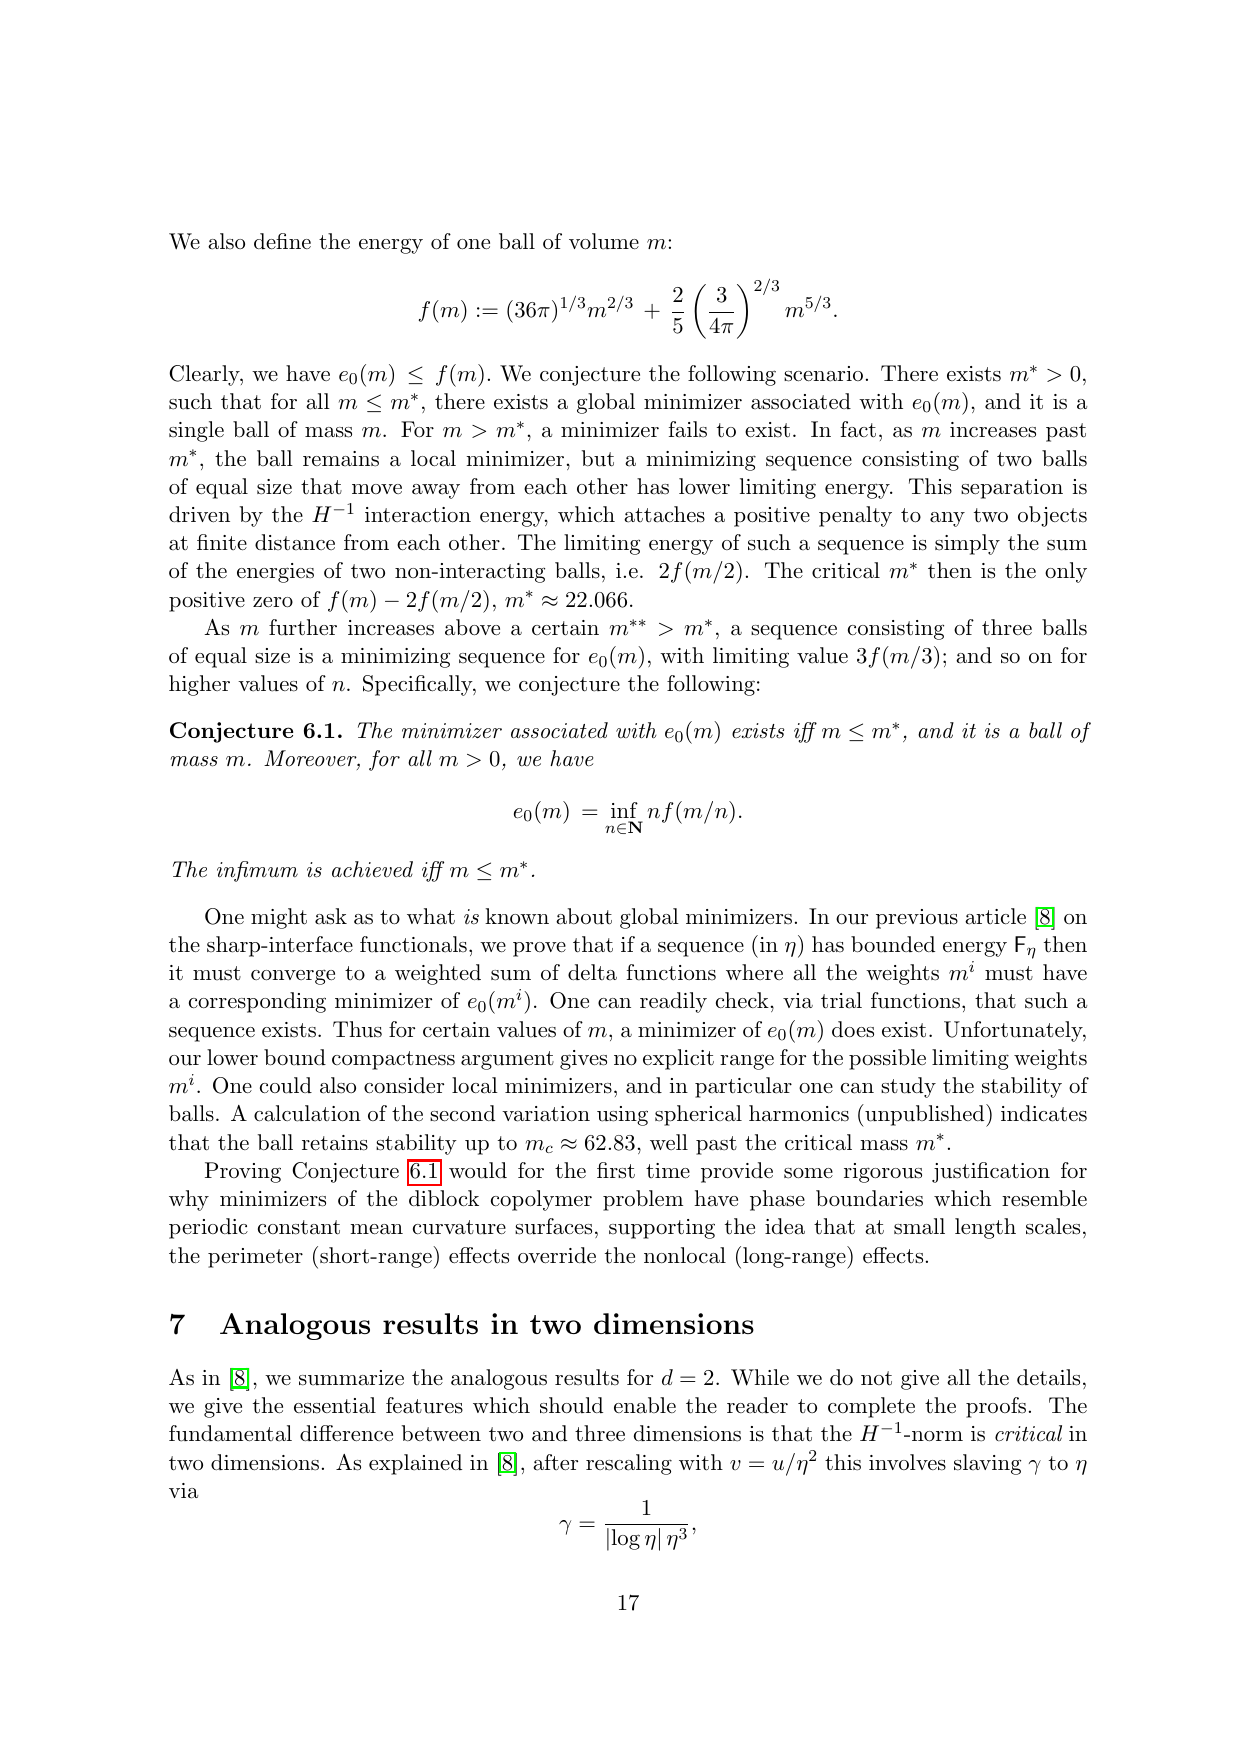
\includegraphics[width=\textwidth,height=0.93\textheight,keepaspectratio]
    {figures/source_page17.png}
\end{center}

\clearpage
\section{The partition theorem}

For $m>0$, define
\[
 G(m):=\inf\left\{\sum_{i\in I}f(m_i):
 I\text{ finite or countable},\ m_i>0,\ \sum_{i\in I}m_i=m\right\}.
\]

\begin{theorem}[exact spherical fragmentation]\label{thm:partition}
For every $m>0$,
\begin{equation}\label{eq:partition}
 G(m)=\min_{n\ge1}F_n(m),\qquad
 F_n(m):=n f(m/n).
\end{equation}
Every minimizing partition is finite and equal: it consists of $n$ copies
of $m/n$ for a minimizing integer $n$.  At a transition precisely two
adjacent equal partitions minimize; otherwise the minimizing partition is
unique up to permutation.
\end{theorem}

\begin{proof}
First fix a maximum number $k$ of positive pieces.  The corresponding closed
simplex is compact.  A minimizer lies in the relative interior of a face;
write $N$ for the number of its positive coordinates.  If $N\ge2$, the
Lagrange equations give
\[
 f'(m_i)=\lambda,\qquad
 f'(s)=\frac13s^{-1/3}(2a+5bs).
\]
Writing $u=s^{1/3}$ shows that $f'(s)=(2a/u+5bu^2)/3$ first decreases and
then increases.  Thus a critical partition has at most two distinct masses.
Moreover
\begin{equation}\label{eq:fpp}
 f''(s)=\frac29s^{-4/3}(-a+5bs),
\end{equation}
so the smaller mass lies on the concave branch.  It cannot occur twice,
since transferring mass between two such coordinates gives a negative
second variation.

It remains to rule out one small mass $x$ and $q\ge1$ copies of a larger
mass $y$.  Put $y=r^3x$ with $r>1$.  The stationarity equation
$f'(x)=f'(y)$ gives
\begin{equation}\label{eq:mixed-x}
 x=\frac{2a}{5br(r+1)}.
\end{equation}
Substitution into \eqref{eq:fpp} yields the exact curvature ratio
\begin{equation}\label{eq:ratio}
 \frac{f''(y)}{|f''(x)|}
 =\frac{2r+1}{r^3(r+2)}<1.
\end{equation}
Along the constraint-preserving variation which adds $t$ to $x$ and
subtracts $t/q$ from each copy of $y$, the second derivative is
\[
 f''(x)+\frac1q f''(y)<0.
\]
Every mixed critical point is therefore a saddle.  Hence every finite
minimum is equal on its positive support.  Minimizing over the possible face
sizes gives $\min_{1\le n\le k}F_n(m)$.

To pass to countable partitions, observe that sufficiently small masses can
always be merged.  If $x+y=s$ and $t=x/s$, then
\begin{align*}
 f(x)+f(y)-f(s)
 &=a s^{2/3}A(t)-b s^{5/3}B(t),\\
 A(t)&=t^{2/3}+(1-t)^{2/3}-1>0,\\
 B(t)&=1-t^{5/3}-(1-t)^{5/3}>0.
\end{align*}
The ratio $A/B$ is continuous and positive on $(0,1)$, is symmetric, and
tends to infinity at both endpoints.  It therefore has a positive minimum
$c$.  Whenever $s<(a/b)c$, the displayed difference is positive.

Given a countable partition, choose a tail whose total mass $s$ is below
this threshold. Repeatedly merge finite partial tails and pass to the limit;
continuity of $f$ gives
\[
 \sum_{i>N}f(m_i)\ge f\left(\sum_{i>N}m_i\right).
\]
The resulting finite partition has no larger energy, so the finite result
proves \eqref{eq:partition}.  An infinite partition cannot attain equality,
because a sufficiently small tail containing two positive masses admits a
strict merge.  Finally, $F_n(m)\to\infty$ as $n\to\infty$, so the discrete
minimum is attained.
\end{proof}

\section{Exact transition masses}

Since
\begin{equation}\label{eq:Fn}
 F_n(m)=a m^{2/3}n^{1/3}+b m^{5/3}n^{-2/3},
\end{equation}
the adjacent branches $F_n$ and $F_{n+1}$ cross exactly at
\begin{equation}\label{eq:mn}
 m_n=\frac ab\,
 \frac{n^{2/3}(n+1)^{2/3}}
 {n^{1/3}+(n+1)^{1/3}}
 =10\pi\,
 \frac{n^{2/3}(n+1)^{2/3}}
 {n^{1/3}+(n+1)^{1/3}}.
\end{equation}
The fraction in \eqref{eq:mn} is strictly increasing in $n$ (the function
$x^2y^2/(x+y)$ is strictly increasing in each positive variable).  Comparing
adjacent branches in \eqref{eq:Fn} therefore gives the complete phase diagram:
with $m_0=0$, $F_n$ is the unique minimum for
\[
 m_{n-1}<m<m_n,
\]
while $F_n=F_{n+1}$ are the only minima at $m=m_n$.  The first thresholds are
\[
\begin{array}{c|rrrrrr}
n&1&2&3&4&5&6\\ \midrule
m_n&22.0670&38.3888&54.3515&70.1996&85.9964&101.7656
\end{array}
\]
In particular $m_1=22.06699868\ldots$ is exactly the source's proposed
$m^*$.  Also $m_n\sim5\pi n$, so optimal component masses converge to $5\pi$.

\section{Strict mass stability and actual ball unions}

The theorem is stable under structure-preserving perturbations.  Suppose
$m_{n-1}<m<m_n$ and $n\ge2$.  At the equal partition $s=m/n$, the constrained
Hessian is
\[
 \frac12 f''(s)\sum_{i=1}^n h_i^2,
 \qquad \sum_i h_i=0.
\]
It is positive.  Indeed, the inflection mass is
\[
 \frac{a}{5b}=2\pi,
\]
and, writing $q=((n-1)/n)^{1/3}\ge2^{-1/3}$,
\[
 \frac{m_{n-1}}n
 =10\pi\frac{q^2}{q+1}>2\pi.
\]
Thus every nontrivial sufficiently small mass-preserving redistribution
strictly raises the energy.  At a transition, each of the two equal branches
has the same within-branch stability, while the droplet count is degenerate.

\begin{corollary}[finite unions of balls]\label{cor:balls}
Among all finite unions of pairwise disjoint balls of total volume $m$, the
infimum of the liquid-drop energy is $\min_nF_n(m)$.  It is approached by
the optimal number of equal balls whose mutual distances tend to infinity.
For $m\le m_1$ a single ball attains the restricted infimum.  For $m>m_1$
the restricted infimum is not attained at finite separation.
\end{corollary}

\begin{proof}
For disjoint balls, perimeter is additive (sphere intersections have zero
surface measure), while every cross-Coulomb term is nonnegative and is
strictly positive for two nonempty components at finite distance.  Hence
\[
 \E\left(\bigcup_{i=1}^N B_i\right)
 \ge\sum_{i=1}^Nf(|B_i|)\ge\min_nF_n(m).
\]
Conversely, translate an optimal equal family so that all mutual distances
tend to infinity.  Every cross term tends to zero, proving equality of the
infima and the attainment claims.
\end{proof}

\section{Why this does not yet prove the full conjecture}

The missing implication is global rather than combinatorial.  For an
arbitrary component $\Omega$ of mass $s$, perimeter favors the ball but the
repulsive Coulomb term favors spreading; one does not know throughout the
necessary range that
\[
 P(\Omega)+D(\Omega)\ge f(s).
\]
Replacing each component by a ball is therefore not an energy-decreasing
operation.  Local shape stability near a ball cannot exclude distant
nonspherical competitors.

Frank and Nam (arXiv:2101.02163) proved existence of minimizers throughout
$0<m\le m^*$ and proved ball uniqueness there conditional on sharp
nonexistence for $m>m^*$.  Their theorem page is reproduced next.  This
pinpoints the obstruction: an arbitrary-shape upgrade of the present result
would solve the still-open global liquid-drop step, not merely strengthen a
partition lemma.

\clearpage
\begin{center}
  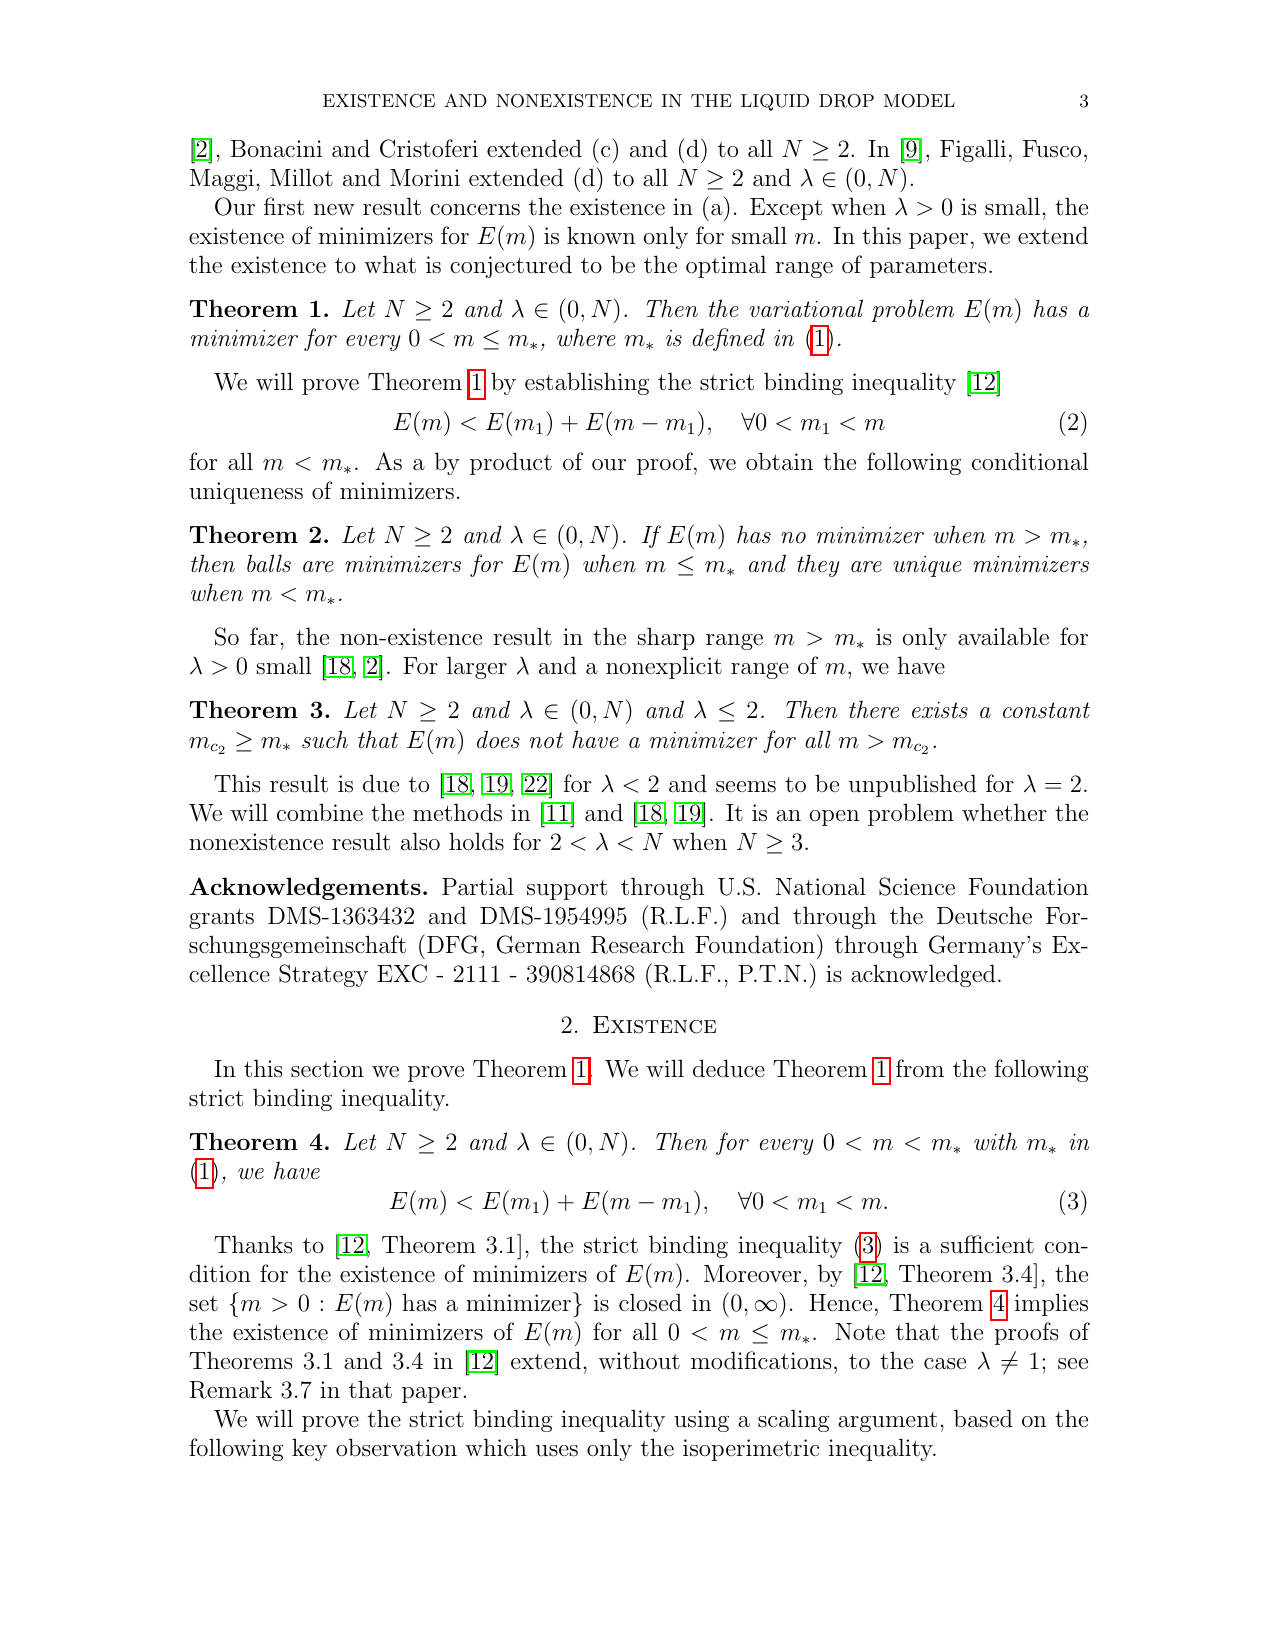
\includegraphics[width=\textwidth,height=0.93\textheight,keepaspectratio]
    {figures/later_page3.png}
\end{center}

\clearpage
\section{Checks, upgrade log, and scope}

\paragraph{Independent checks.}
The companion script verifies $a/b=10\pi$, the first 79 transition
identities and their strict ordering, the curvature ratio
\eqref{eq:ratio} on a logarithmic grid, and 16,000 random finite partitions
against the exact envelope.  These computations are diagnostic only; the
proof above is analytic.

\paragraph{Upgrade log.}
The investigation made six focused passes: (1) a numerical search over
one-small/many-large partitions; (2) the exact negative second-variation
argument excluding every mixed critical point; (3) the uniform small-tail
merge extending the theorem to countable partitions; (4) the closed-form
transition diagram and strict mass-redistribution stability; (5) the
positive-cross-interaction extension to actual finite unions of balls; and
(6) an arbitrary-shape upgrade attempt, which reduces to the known open
global ball-optimality/sharp-nonexistence problem.

\paragraph{Literature boundary and novelty.}
Bounded primary-source searches through 11 August 2026 found the source,
Frank--Nam's 2021 existence and conditional-uniqueness result, prior
large-mass nonexistence bounds, and a 2026 improvement of that bound.  No
source located in the search stated the finite/countable equal-fragmentation
theorem with its complete phase diagram.  The argument is elementary enough
that it may be implicit or folklore; the packet should therefore be treated
as a candidate substantial partial result, not a priority claim.

\paragraph{Human review.}
Check the relative-face minimization step, the mixed-point curvature ratio,
and the small-tail merge.  Also verify that the intended restricted class in
Corollary~\ref{cor:balls} consists of disjoint spherical components; no claim
is made for general shapes.

\begin{thebibliography}{9}
\bibitem{CP}
R.~Choksi and M.~A. Peletier,
\emph{Small volume fraction limit of the diblock copolymer problem II:
diffuse-interface functional}, arXiv:1004.4271.

\bibitem{FN}
R.~L. Frank and P.~T. Nam,
\emph{Existence and nonexistence in the liquid drop model},
arXiv:2101.02163.

\bibitem{FKN}
R.~L. Frank, R.~Killip, and P.~T. Nam,
\emph{Nonexistence of large nuclei in the liquid drop model},
arXiv:1604.03231.
\end{thebibliography}

\end{document}
